%TODO: Add benchmarks from .csv

%% Preamble
\documentclass{beamer}
\usetheme{Warsaw}
\usepackage{url}

\AtBeginSection[]
{
	\begin{frame}
		\frametitle{Table of Contents}
		\tableofcontents[currentsection]
	\end{frame}
}

\title{Parallel computing in Julia}
\author{Jasper Boomer}
\titlegraphic{
\includegraphics[width=.3\textwidth]{figures/logo.png}}

%% Document
\begin{document}
	\frame{\titlepage}
	\section{Introduction}

	\begin{frame}{General}
		\begin{block}{Julia is:} 
		\begin{itemize}
			\item{Free \& Open source (MIT licensed)}
			\item{Development started in 2009, v0.1 in 2012}
			\item{General purpose high-level dynamic programming language}
			\item{Designed for parallelism \& distributed computation}
			\item{Core written in C/C++, STL in Julia}
			\item{JIT Compiled}
			\item{Optimized for speed of calculation}
		\end{itemize}
		\end{block}
	\end{frame}
	
	\begin{frame}{Benchmarks}
		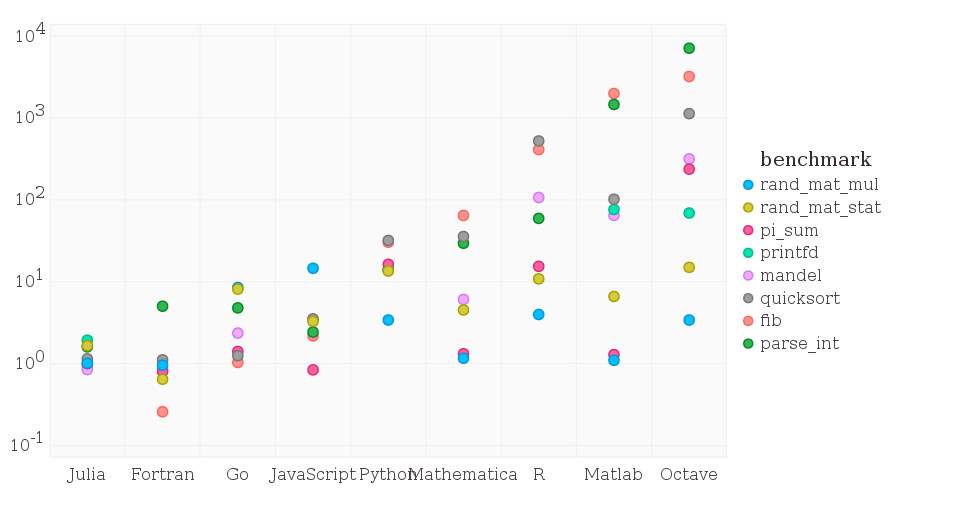
\includegraphics[width=\textwidth]{figures/benchmarks.jpg}
	\end{frame}

	\begin{frame}[fragile]{Some features(1)}
		\begin{block}{Examples}
			\begin{semiverbatim}
			julia> [i*2 for i=1:5]
			[1 4 6 8 10]
			
			julia> function printargs(args...)
			         for a in args
		 	           println(a)
			         end
			       end
			printargs (generic function with 1 method)

			julia> map(x->(x\%3==0), [3 4 12])
			[true, false, true]
			\end{semiverbatim}
		\end{block}
	\end{frame}

	\begin{frame}[fragile]{Macros}
		Expressions are Julia objects. These can be modified and then run.
		\begin{block}{@time macro}
			\begin{semiverbatim}
			macro time(d::Expr) 
			  local t0 = time()
			  local val = \$d
			  tocal t1 = time()
			  println("elapsed time: ", t1-t0, " seconds")
			  return val
			end

			julia> @time rand(100,00)
			elapsed time 0.00679384 seconds
			100x100 Array\{Float64\}
			\end{semiverbatim}
		\end{block}
	\end{frame}

	\section{Tasks}

	\begin{frame}{Tasks vs Functions}
		\begin{columns}[c]
			\column{0.5\textwidth}
				\textbf{Functions (Sub-routines)} \\
				Call / Return
			\column{0.5\textwidth}
				\textbf{Tasks (Co-routines)} \\
				Yielding to other tasks (saving state)
		\end{columns}
	\end{frame}

	\begin{frame}{Example: Sieve of Erasthothenes}
		Sieve
	\end{frame}

	\section{Low-level parallelism in Julia}
	%TODO: Stukje over feeder task (zie parallel computing in docs)

	\begin{frame}{General}
		\begin{itemize}
			\item{No native threads (yet?)}
			\item{No need for mutex locks etc.}	
			\item{Uses message passing interface to run on different processors}
			\item{Implementation of message passing is one-sided}
		\end{itemize}

	\end{frame}
	
	\begin{frame}[fragile]{Worker processes}
		Syntax:
		\begin{semiverbatim}
			julia -p N [filename]
		\end{semiverbatim}
		\begin{itemize}
			\item{Launches \verb+N+ worker processes}
			\item{Runs \verb+filename+ or interactive session}
			\item{Workers are numbered $2:N+1$}
			\item{Can run on multiple cores or cluster of computers}
		\end{itemize}
	\end{frame}

	\begin{frame}[fragile]{Remote calls \& references}
		\begin{block}{Executing statements on specific worker processes}
		\begin{semiverbatim}
		julia -p 2
		julia> r = remotecall(2, sin, pi/4)
		RemoteRef(3,1,2) 

		julia> fetch(r)
		0.7071067811865475

		julia> remotecall\_fetch(2, myid)
		2
		
		julia> @spawn cos(pi/4) 
		RemoteRef(3,1,3)
		\end{semiverbatim}
		\end{block}
	\end{frame}

	\begin{frame}[fragile]{Parallel for loops(1)}
		\begin{block}{Reduction function}	
		\begin{semiverbatim}
		rand\_number = @parallel (+) for i=1:10000000
		  rand()
		end
		\end{semiverbatim}
		\end{block}
	\end{frame}

	\begin{frame}{Parallel for loops(2)}
		Example: \\
		parallel computation of $\pi$
		\begin{columns}[c]
			\column{0.5\textwidth}
			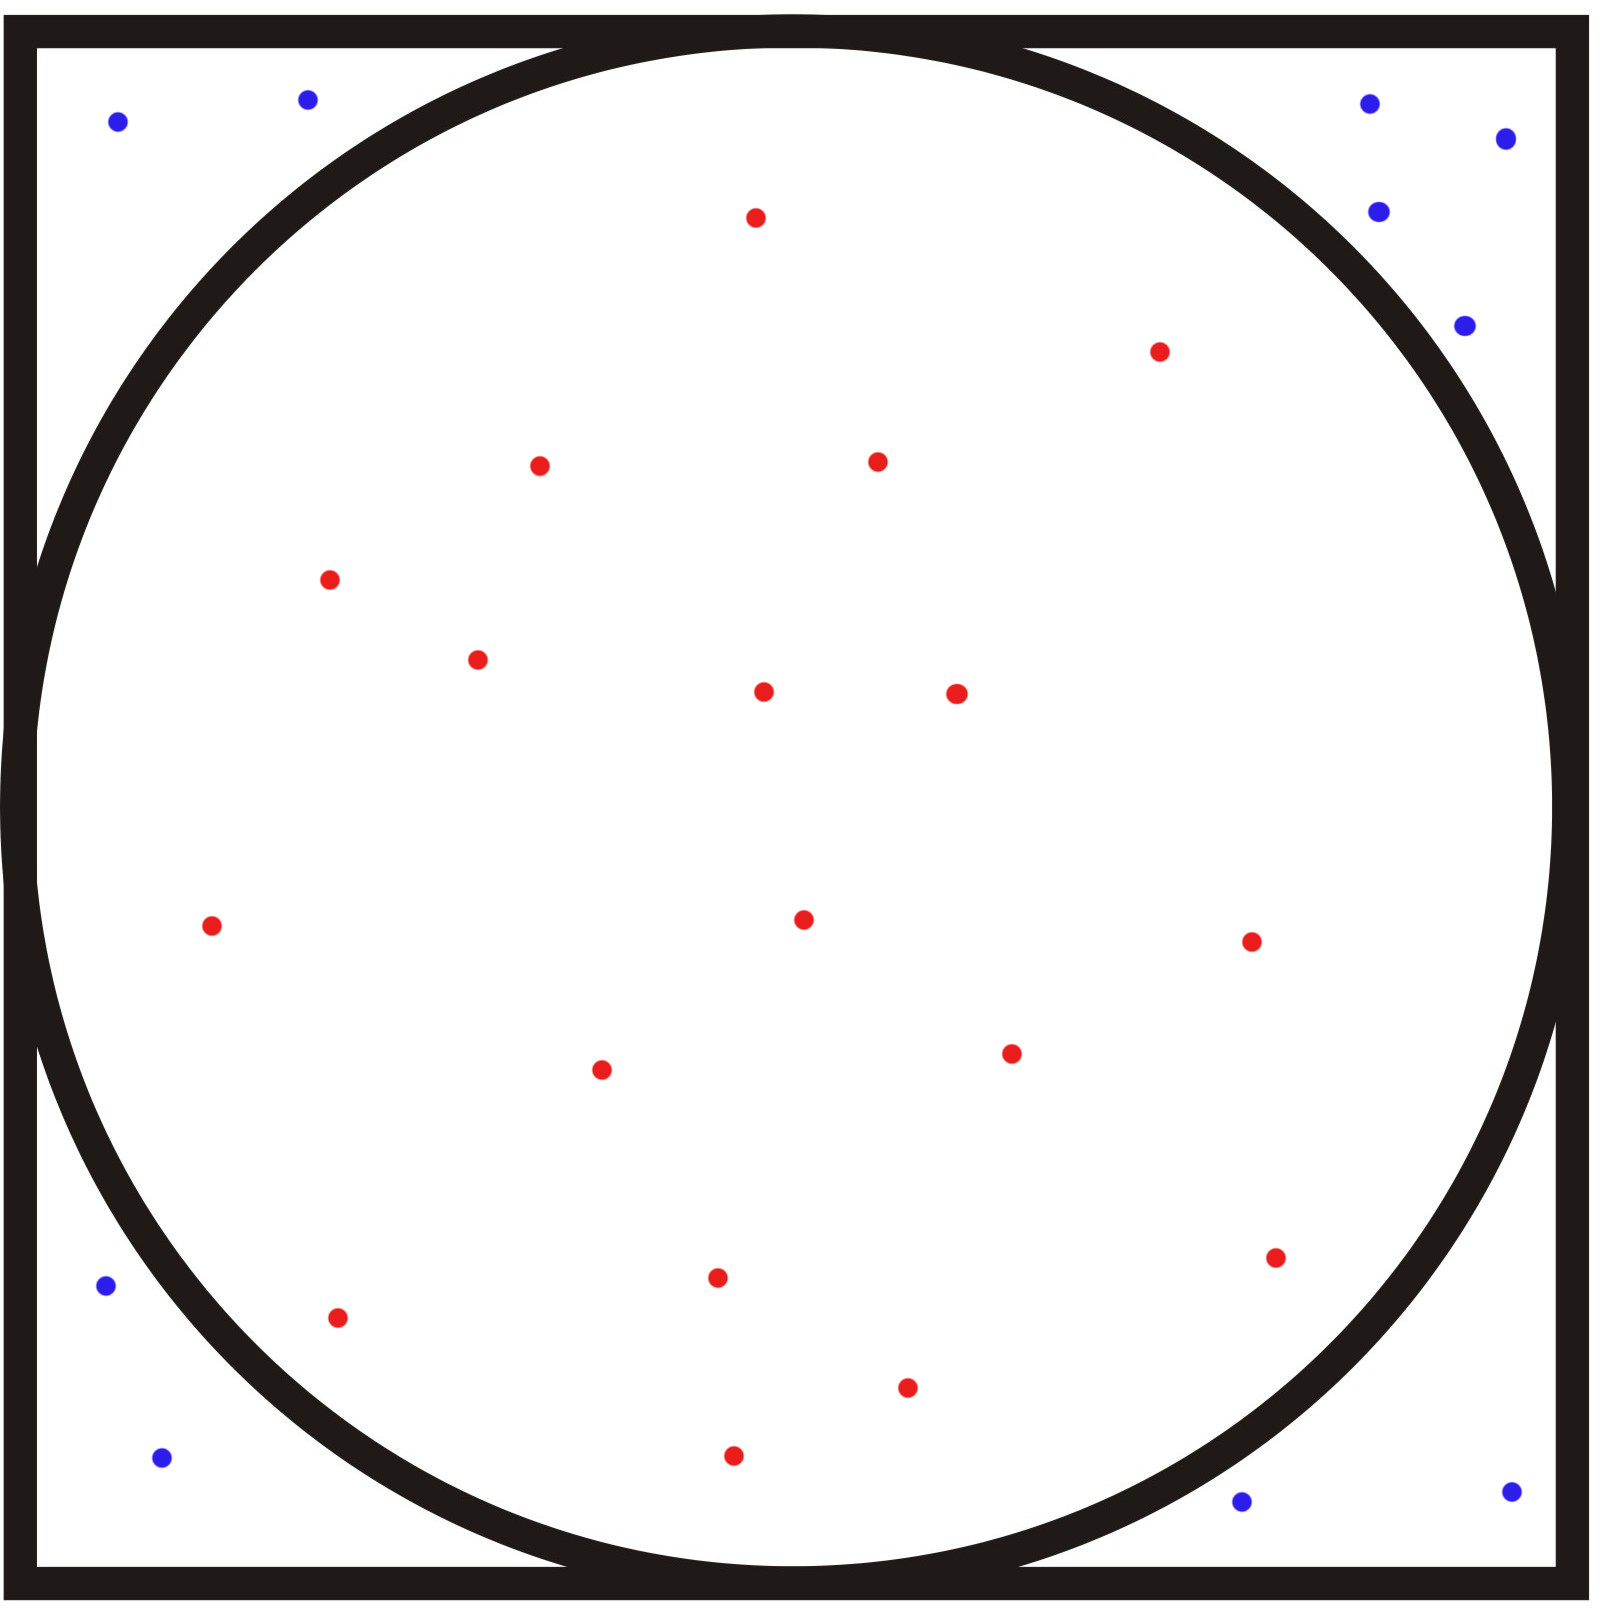
\includegraphics[height=4cm]{figures/square_circle.jpg}
			\column{0.5\textwidth}
			Draw random points, get $\pi$ from ratio of points in the circle.
			\begin{equation*}
				\begin{array}{rcl}		
					A_{rect} & = & (2r)^2 = 4r^2 \\
					A_{circle} & = & \pi r^2 \\
					\pi & = & 4\frac{A_{circle}}{A_{rect}}
				\end{array}
			\end{equation*}
		\end{columns}
	\end{frame}

	\section{Distributed arrays}

	\begin{frame}[fragile]{Distributed Arrays}
		\begin{block}{Constructor}
		\begin{semiverbatim}
		DArray(init, dims[, procs, dist])
		\end{semiverbatim}
		\end{block}
		\begin{block}{Example with 8 workers:}
		\begin{semiverbatim}
		julia> d = DArray(I->rand(length(I[1]),length(I[2])),
											(80, 80), 
											[2:9], 
											[4,2]);	
		
		julia> remotecall\_fetch(2,localindexes,d)
		(1:20, 1:40)
		
		julia> remotecall\_fetch(7,localindexes,d)
		(21:40, 41:80)
		\end{semiverbatim}
		\end{block}
	\end{frame}

	\begin{frame}{Example: Mandelbrot Set}
		\begin{columns}[c]
		\column{.5\textwidth}
			
\includegraphics[height = 4cm]{figures/mandel_zoom.jpg}	
		\column{.5\textwidth}
			\begin{equation*}
			\begin{array}{rcl}
				c\in\mathbb{C}: & & \\
				z_0 & = & 0	\\
				z_{n+1} & = & z_n^2 + c
			\end{array}
			\end{equation*}
			Set of $c$ for which orbit of z around 0 remains bounded. Colours indicate escape time.
		\end{columns}
	\end{frame}
	
	\section{Last words}
	
	\begin{frame}{Links}
		\begin{itemize}
			\item{\url{http://julialang.org/}}
			\item{\url{https://github.com/jboomer/parallel-julia/}}
		\end{itemize}
	\end{frame}
	
	\section{Questions}

\end{document}
